\chapter{Neural Networks: an introduction}
The idea of \textbf{neureal network (NN)} was introduced in the late 50s, in order to implement algorithm which could try to mimic the brain functionalities. They were very used in 80s, but their popularity decreased in the late 90s. Two determinant factors have aided the resurgence of such  technologies: the increasing in the quantity of data, and the increasing in computation capacity. For example, Neural Networks are used, among the others tasks, for performing classification.
We have understood that a linear hypotesis is not suitable for such a task, then nonlinearity is needed.\\
Now, let us imagine we want to build a model for classifying in a binary way, some images in two classes: CAR, NO CAR. An image is in general composed of pixels. Can we use \textit{logistic regression} for doing image classification? Let us consider a training set made up of $64\times{64}$ images, then 4096 pixels which is the same number for the parameter if we have a gray-scale image. If we have RGB images, the number of parameters grows by a $3$ factor, that is a number of parameters equal to $n=12288$, a huge number that makes highly unsuitable the logistic regression models. In this situation a neural network of some type is used.

\section{Ideas underlying neural networks}
Before going on through the discussion of (Artificial) Neural Networks, we have to just mention how a biological neuron is made.

\begin{figure}[h]
    \centering
    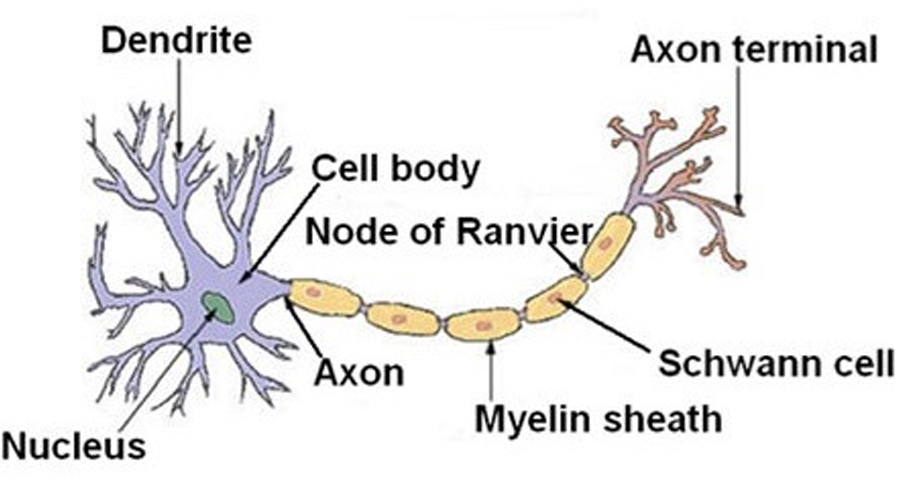
\includegraphics[scale=0.5]{img/bio_neuron.png}
\end{figure}
\noindent
Three are the main components of a neuron:
\begin{enumerate}
    \itemsep-0.2em
    \item Some inputs wires (\textbf{Dendrites})
    \item A \textbf{Nucleus} which is the \textit{computational unit}
    \item An output wire (\textbf{Axon})
\end{enumerate}
Clearly such a type of cells are connected each other by mean of \textit{synapses} realized by neutrotransmitters. \\
The \textbf{artificial neural newtork} has exactly the same structure of a biological one whose building blocks are some \textit{artificial neurons} made up of the same three basic elements, since it has got: (i) some inputs which are the features, (ii) a computation unit that performs a weighted sum of the features, (iii) an output which is the result of an \textbf{activation function} which often can be a sigmoid. [From this point we can see the strong relationship with the logistic regression.] Other activation functions can be used, besides another example is the \textbf{ReLU}.

\begin{figure}[h]
    \centering
    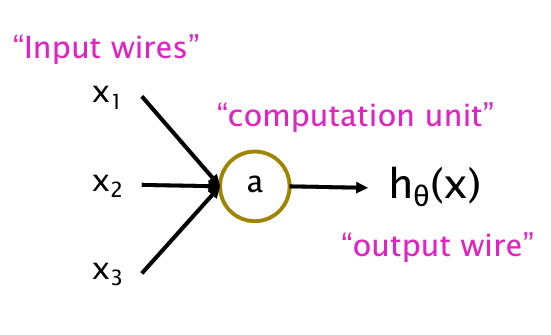
\includegraphics[scale=0.7]{img/artificialneuron.png}
    \caption{Structure of an artificial neuron}
\end{figure}

\subsection{Notation} 
In the following some notation is introduced that will be used in the remaining part of the course dealing with neural networks. When we put together some artificial neurons, what we obtained in general is a \textbf{multilayer perceptron} or \textit{classical NN}. The \textit{layer 0} is the input layer, the following are numbered as first, second layer and so on. In each layer we can find one or more computational units. For example the first layer of the showed NN has 3 computational units (without considering the unit 0 which is associated to the bias). The notation $a_i^{[j]}$ indicates the \textbf{activation} in the \textbf{i-th unit} in the \textbf{$j$-th level} of the network, while $\Theta^{[j]}$ is the weighting matrix for the  $j$-th layer of the network.\footnote{
    The intermediate layers of a neural network are called \textbf{hidden layers} since the output produced is hidden and are generated by linear and non linear combination of the features.
}
Usually also the input are renamed as \textit {zero-layer activation}, then are indicated with $a_i^{[0]}$. For the presented MLP\footnote{
    multilayer perceptron
} let us try to write all of the activation of each layer:
\begin{align*}
    &a_1^{[1]} = g(\Theta_{10}^{[1]} a_0^{[0]} + \Theta_{11}^{[1]} a_1^{[0]}+\Theta_{12}^{[1]}a_2^{[0]}+\Theta_{13}^{[1]}a_3^{[0]})=g(z_1^{[1]})\\
    &a_2^{[1]} = g(\Theta_{20}^{[1]} a_0^{[0]} + \Theta_{21}^{[1]} a_1^{[0]}+\Theta_{22}^{[1]}a_2^{[1]}+\Theta_{23}^{[1]}a_3^{[0]})=g(z_2^{[1]})\\
    &a_3^{[1]} = g(\Theta_{30}^{[1]} a_0^{[0]} + \Theta_{31}^{[1]} a_1^{[0]}+\Theta_{32}^{[1]}a_2^{[0]}+\Theta_{33}^{[1]}a_3^{[0]})=g(z_3^{[1]})\\
    &a_1^{[2]} = g(
        \Theta_{10}^{[2]}a_0^{[1]}+
        \Theta_{11}^{[2]}a_1^{[1]}+
        \Theta_{12}^{[2]}a_2^{[1]}+
        \Theta_{13}^{[2]}a_3^{[1]} 
    )=g(z_1^{[2]})
\end{align*}
\noindent
In this case the weighting matrices are for the first layer $\Theta^{[1]}\in\mathbb{R}^{3,4}$, for the second layer is $\Theta^{[2]}\in\mathbb{R}^{1,4}$.

\subsection{Different types of NN for different types of purposes}
A neural network can be used either for binary or multiclass classification. In the former case the last layer has got one neuron whose activation is 0 or 1, in the latter case we have a neuron for each class in a level that is (how we will see) the \textit{softmax layer}. Moreover a neural network is said to be \textbf{shallow} (typically) when it is made up of a number of layers which is less than seven, otherwise we have a \textbf{deep neural network}.

\begin{figure}[h]
    \centering
    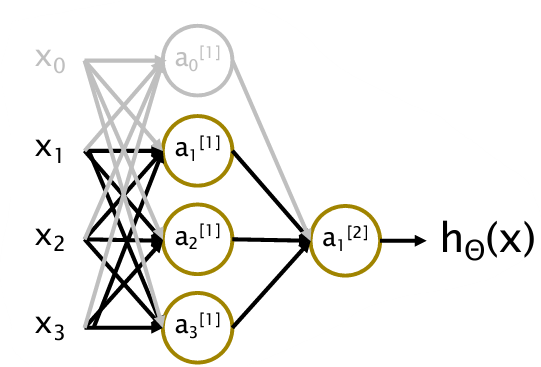
\includegraphics[scale=0.6]{img/neuron_spec.png}
\end{figure}

\section{Logistic regression as a NN}
If we better analyse the structure of a neuron and the path going from the input to the output of it, we will discover that it is something very similar to what we have seen in the case of logistic regression, where we have combined a linear part with a non linear one in order to correctly perform the (binary) classification task.\\
Now, let us suppose we want to perform a binary classification a set of images, in particular we want distinguish when they are cars or not. Can we use logistic regression in order to perform such a task? NO! It could be very slow and inefficient: a logistic regression (that is a single neuron) cannot perform in a good way such a task, then a neural network is used in this case. The next step is: how can we represent an image as a vector of features? We know that a gray-scale image can be represented as a matrix of numbers in the range [0-255], if the image is RGB we have a different matrix for each one of the channel R, G and B. We can turn the matrix into a vector by simply unrolling it row by row, in a way that each single pixel of each one of the channel is a feature for our classification problem. This example was just to present the problem of \textbf{vectorization}, that in the field of neural network is a very common operation which is done on the data in order to make them suitable for network itself.\\

\noindent
We have seen in the logistic regression that our \textbf{predicted value} $\hat{y}$ (which was the hypotesis), is nothing but the result of a sigmoidal function applied to the linear combination $w^T{x}+b$, where $w$ are the weights, $b$ is the bias while $x$ is the feature vector. Then we have that: 
\begin{equation}
    \hat{y}=a=\sigma(w^T{x}+b)
\end{equation}
How we mentioned, this is exactly the work performed by a neuron from the inputs to the output. Furthermore, we have seen that for the logistic regression a different cost function must be considered in order not to dealing with \textit{non-convex optimization problem}. For the description of the logistic regression as a single-neuron NN, nothing change a part from few differences in the notation. In fact we indicate the hypotesis $h_\theta(x)$, with the \textit{predicted value} $\hat{y}$, while the $\theta_i$ parameters are split in weights $w$ and a single bias $b$. Another difference we can find in the field of NN, is that the partial derivatives of the functional $J$ to be minimized with respect to the weights/bias, that is 
\begin{equation}
    \frac{\partial{J}}{\partial{w}}, \quad 
    \frac{\partial{J}}{\partial{b}}
\end{equation}
are denoted simply with $dw$ and $db$, in order to make lighter the notation. The \textit{gradient descent step} in order to decrease the functional becomes:
\begin{align*}
    &w = w - \alpha\ {dw}\\
    &b = b - \alpha\ {db}
\end{align*}
Now, \textbf{How can we compute the partial derivatives?} For sure, we can say that no explicit analytic calculation are performed, instead a very powerful tool that is the \textbf{automatic differentiation} leveraging on the so-called \textbf{computation graph} is used. The main concept behind it is to express a function by using \textit{intermediate auxiliary variables} and computing the derivatives by using the \textbf{Leibnitz's Chain Rule}.

\section{Automatic differentiation and computation graph}
Suppose we have a function
\begin{equation}\label{eq:exJ}
    J(a,b,c)=3(a+bc)
\end{equation}
we want to compute the ppartial derivatives of $J$ with respect to the three variables $a,b,c$. We can introduce some intermediate variables which can be called
\begin{equation*}
    u=bc \quad  v=a+u
\end{equation*}
Our function $J$ becomes: $J=3v$. In this way we have split the original function in trhee different simpler functions. This procedure can be graphically represented as shown in the figure:

\begin{figure}[h]
    \centering
    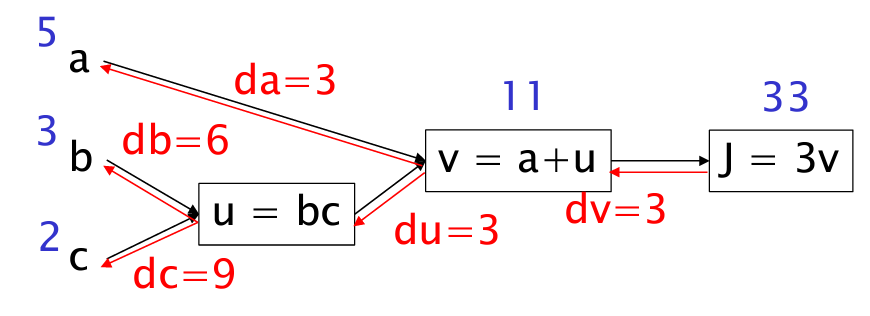
\includegraphics[scale=0.5]{img/computation_graph.png}
    \caption{Computation graph for $J=3(a+bc)$}
\end{figure}
\noindent
In particular from the input $a,b,c$, we can compute the value of the intermediate variable $u$, which can be used for obtaining $v$, finally we can compute $J$. This path from $(a,b,c)\to{J}$ is called \textbf{Forward Propagation}. Now, what about the partial derivatives? We can proceed step by step, doing an inverse path from $J\to(a,b,c)$, intuitively such a path is the \textbf{Backward propagation}, here the \textit{Chain rule} is used in order to carry out 'gradually' the computation of the partial derivatives.
The following steps are done:
\begin{align*}
    &\frac{\partial{J}}{\partial{v}}\doteq{\color{red}\mathbf{dv}}=\mathbf{\color{red}3} \quad
    \frac{\partial{J}}{\partial{u}}\doteq{\color{red}\mathbf{du}}=
    \frac{\partial{J}}{\partial{v}} \frac{\partial{v}}{\partial{u}} = 3 \cdot 1 = \mathbf{\color{red}3}\\
    &\frac{\partial{J}}{\partial{a}} \doteq{\color{red}\mathbf{da}}=
    \frac{\partial{J}}{\partial{v}} \frac{\partial{v}}{\partial{a}} = \mathbf{\color{red}3} \quad
    \frac{\partial{J}}{\partial{b}}\doteq{\color{red}\mathbf{db}}=
    \frac{\partial{J}}{\partial{v}}\frac{\partial{v}}{\partial{u}}\frac{\partial{u}}{\partial{b}}=3\cdot{1}\cdot{c}=3c=\mathbf{\color{red}6}\\
    &\frac{\partial{J}}{\partial{c}}\doteq{\color{red}\mathbf{dc}}=
    \frac{\partial{J}}{\partial{v}}\frac{\partial{v}}{\partial{u}}\frac{\partial{u}}{\partial{c}}=3\cdot{b}=\mathbf{\color{red}9}
\end{align*}
The procedure we have just shown is THE way in which are computed the derivatives in the field of Neural Network. Clearly, the same reasoning we have done for the functional (\ref{eq:exJ}) can be repeated for the \textit{loss function} used for the case of logistic regression. The figure below shows the final result of forward and backward propagation applied for the \textbf{cross-entropy loss function}.
\begin{figure}[h]
    \centering
    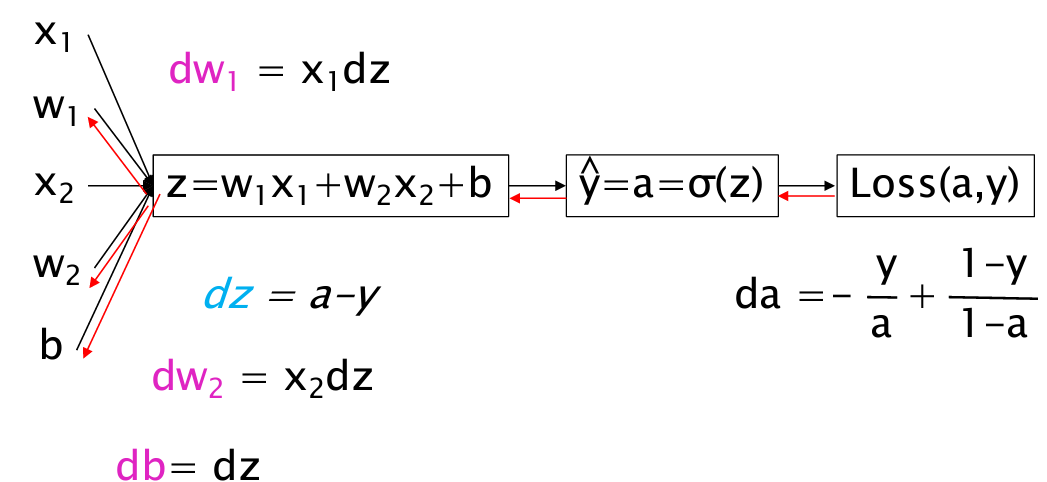
\includegraphics[scale=0.5]{img/compgraph_Loss.png}   
\end{figure}

\subsection{Feedback and Backward propagation for Logistic Regression}
For a single training sample we have that the feedback and backward propagation mathematical steps are the following:
\begin{multicols}{2}
    \noindent
    \textbf{FORWARD PROPAGATION}
    \begin{align*}
        &z_i=w^T{x^{(i)}}+b \quad \text{(linear part)}\\
        &\hat{y}_i=a_i=\sigma(z_{i})   \quad \text{(activation)}\\
        &J_{i}=-[y_{i}\log{a_{i}}+(1-y_{i})\log(1-a_{i})] \\
        & \quad \quad \text{(cost function)}
    \end{align*}
    \newcolumn\\
    \noindent
    \textbf{BACKWARD PROPAGATION}
    %\begin{align*}
        %&z=w^T{X}+b \quad \text{(linear part)}\\
        %&\hat{y}=a=\sigma(z)   \quad \text{(activation)}\\
        %&J=-\frac{1}{m}[y\log{a}+(1-y)\log(1-a)] \\
        %& \quad \quad \text{(cost function)}
    %\end{align*}
    \begin{align*}
        &dz_i = a_i-y_i\\
        &dw_i={x^{(i)}}{dz_i}\\
        &db_i=dz_i
    \end{align*}
\end{multicols}
\noindent
Whether we extend such computations to the whole dataset, we have matrices and vectors instead of vectors and scalars. In particular:
\begin{multicols}{2}
    \noindent
    \textbf{FORWARD PROPAGATION}
    \begin{align*}
        &z=w^T{X}+b \quad \text{(linear part)}\\
        &\hat{y}=a=\sigma(z)   \quad \text{(activation)}\\
        &J_{i}=-1/m \sum [y\log{a}+(1-y)\log(1-a)] \\
        & \quad \quad \text{(cost function)}
    \end{align*}
    \newcolumn\\
    \noindent
    \textbf{BACKWARD PROPAGATION}
    %\begin{align*}
        %&z=w^T{X}+b \quad \text{(linear part)}\\
        %&\hat{y}=a=\sigma(z)   \quad \text{(activation)}\\
        %&J=-\frac{1}{m}[y\log{a}+(1-y)\log(1-a)] \\
        %& \quad \quad \text{(cost function)}
    %\end{align*}
    \begin{align*}
        &dz = a-y\\
        &dw= \frac{1}{m} (X^T{dz^T})\mathbf{1}\\
        &db=\frac{1}{m}(\mathbf{1}^T{dz})
    \end{align*}
\end{multicols}
\noindent
Where $\mathbf{1}$ is a column vector with all ones. After having performed the forward and backward steps, both weights and bias must be updated as follows: 
\begin{equation}
    w:=w-\alpha\cdot{dw} \quad b:= b-\alpha\cdot{db}
\end{equation}
Such steps must be repeated until convergence (in some sense). Keep always in mind that $dw$ and $db$ are the partial derivatives of the cost function with respect to the weights and bias.

\section{Training Neural Networks}
Till now we have seen the optimization procedure of the \textit{logistic regression} as a single neuron. However, we know that a neural network is made up of several layers which in turn are composed of several neurons (computational units). The objective here is to understand how we can generalize the \textbf{optimization procedure} in the case when the whole neural network must be trained (in particular the parameters for each neuron, for each layer must be computed).

\begin{figure}[h]
    \centering
    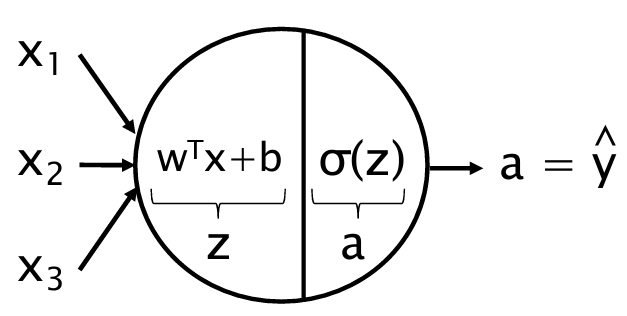
\includegraphics[scale=0.4]{img/single_log_neuron.png}
    \caption{Single neuron in form of logistic regression}
\end{figure}
\noindent
We are going to proceed step by step starting from a single neuron, going to the whole layer analyzing both the forward and backward propagations aimed to generalize the gradient descent algorithm to the whole network. For sake of simplicity but without loss of generality, the analysis has been conducted on a 2-layer NN. In the following the activation function will be indicated with $g$  in order to generalize to the use of different functions which can be used.

\subsection{Forward propagation}

\subsubsection{Single neuron, single sample}
\begin{multicols}{2}
    \begin{center}
        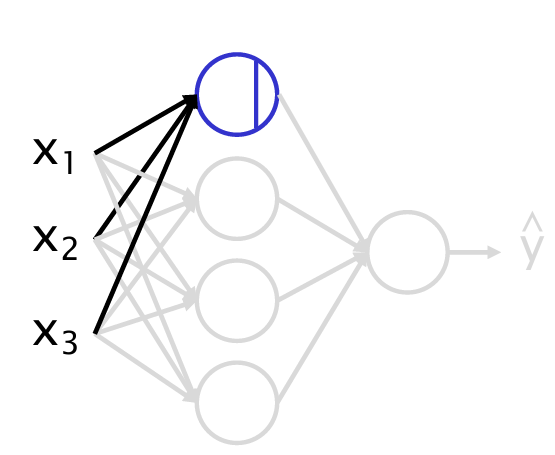
\includegraphics[scale=0.5]{img/2L_single.png}
    \end{center}
    \newcolumn
    A single neuron of the layer is considered, which clearly has his own weights and bias.
    \begin{equation} \label{eq:single_neuron}
        \begin{aligned}
            &z_1^{[1]}=w_1^{[1]T}{x}+b_1^{[1]}\\
            &a_1^{[1]}=g(z_1^{[1]})
        \end{aligned}
    \end{equation}
    The function $g$ can be something different with respect to a sigmoid. Only one sample $x$ of the dataset is considered.
\end{multicols}

\subsubsection{Single Layer, single sample}
\begin{multicols}{2}
    \begin{center}
        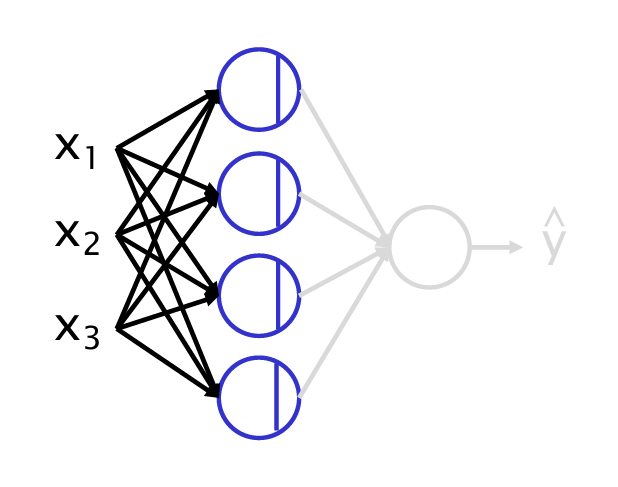
\includegraphics[scale=0.45]{img/2L_layer.png}
        \vspace{-0.5cm}
    \end{center}
    Considering all the neurons in the first layer, we have the (\ref{eq:single_neuron}) repeated four times, that is: 
    \begin{equation*}
        \begin{aligned}
            &z_i^{[1]}=w_i^{[1]T}{a^{[0]}}+b_i^{[1]}\\
            &a_i^{[1]}=g(z_i^{[1]})
        \end{aligned}, \quad i=1,...,4
    \end{equation*}
    Here the only difference is that we have indicated in terms of activations the input. In a more compact form we can say that:
    \begin{equation}
        \begin{aligned}
            &z^{[l]}=W^{[l]}a^{[l-1]}+b^{[l]}\\
            &a^{[l]}=g(z^{[l]})
        \end{aligned}
    \end{equation}
    where $l$ indicates the $l$-th layer of the network.
 \end{multicols}

\subsubsection{Single layer, whole dataset}
Till now we have seen the \textit{forward step} for a single neuron and for a layer of the network. What if considering the whole dataset instead of a single sample? The vector $z$ of the linear combination becomes a matrix in which the \textbf{$i$-th row} contains the linear combination for the \textbf{$j$-th} sample of the activation of the past layer. We have:
\begin{equation}
    \begin{aligned}
        &Z^{[l]}=W^{[l]}A^{[l-1]}+b^{[l]}\\
        &A^{[l]}=g^{[l]}(Z^{[l]})
    \end{aligned}
\end{equation}
Here is noticeable that the activation function can be different for each level of the network. This is the reason why we put the $l$ superposed also on the $g$.
\subsection{Backward propagation}
For the case of backward propagation we give directly the result in the most general case in which the loss function is even different than the \textit{cross-entropy}. Then, we have:
\begin{equation}
    \begin{aligned}
        &dZ^{[l]}=dA^{[l]}.*g^{[l]'} \ Z^{[l]}\\
        &dW^{[l]}=\frac{1}{m} (dZ^{[l]}A^{[l-1]T})\\
        &db^{[l]}=\frac{1}{m} \text{sum}({dZ^{[l]}})=\frac{1}{m}dZ^{[l]}\mathbf{1}\\
        &dA^{[l-1]}=W^{[l]T} dZ^{[l]}
    \end{aligned}
\end{equation}
For the output layer $dA^{[L]}=A^{[L]}$. The gradient step must be performed for each layer once all the derivatives have been computed: 
{\large{
    \begin{equation}
        W^{[l]}:= W^{[l]}-\alpha\cdot{dW^{[l]}} \quad    b^{[l]}:=b^{[l]}-\alpha\cdot{db^{[l-1]}}
    \end{equation} 
}}
The whole procedure of forward and backward propagation can be schematically represented by using a block diagram: 

\begin{figure}[h]
    \centering
    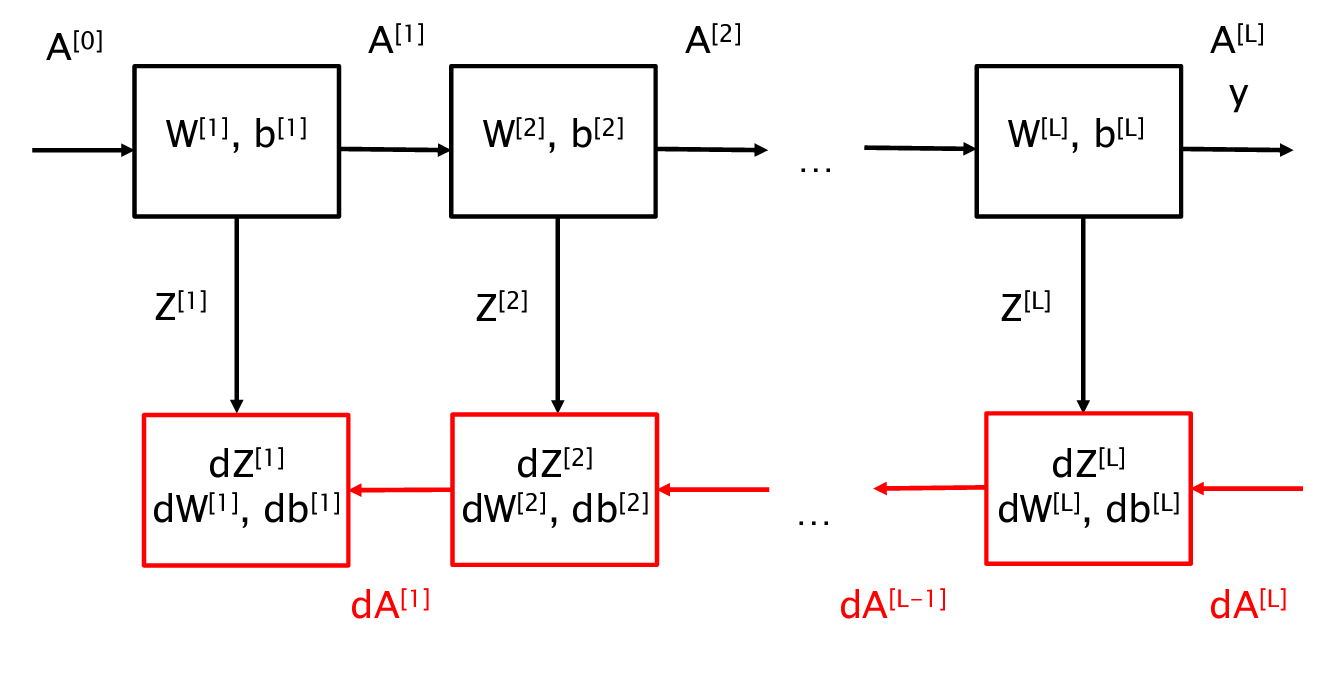
\includegraphics[scale=0.5]{img/block_diagram_GD.png}
    \caption{Block diagram for the GD}
\end{figure}

\section{Activation functions}
At different layers of a neural network, different activation functions can be used. Till now we have seen the sigmoid, since it is the one arising in the case of \textit{logistic regression}. Other choices can be done according to the needed convergence property and the task to be performed. The most common used activation functions are reported in the figure below (in the description there is also the definition).

\begin{figure}[h]
    \centering
    \subfigure[$\sigma(z)={1}/{(1+e^{-z}})$]{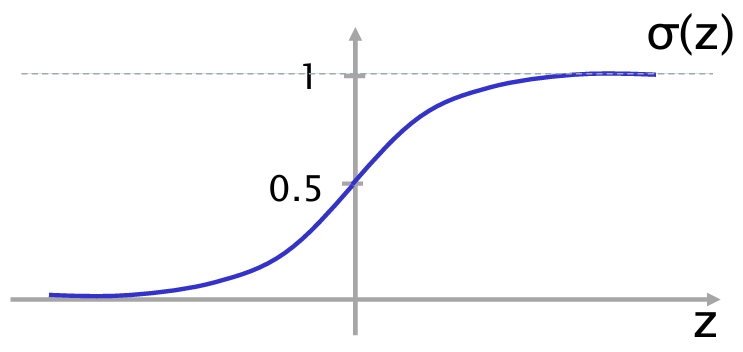
\includegraphics[scale=0.45]{img/sigmoid.png}}
    \subfigure[$\tanh(z)=(e^z-e^{-z})/(e^{z}+e^{-z})$]{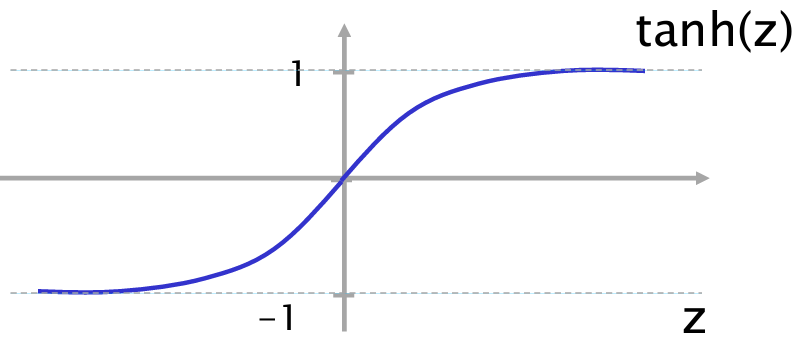
\includegraphics[scale=0.45]{img/tanh.png}}
    \subfigure[$\text{ReLU}(z)=\max(0,z)$]{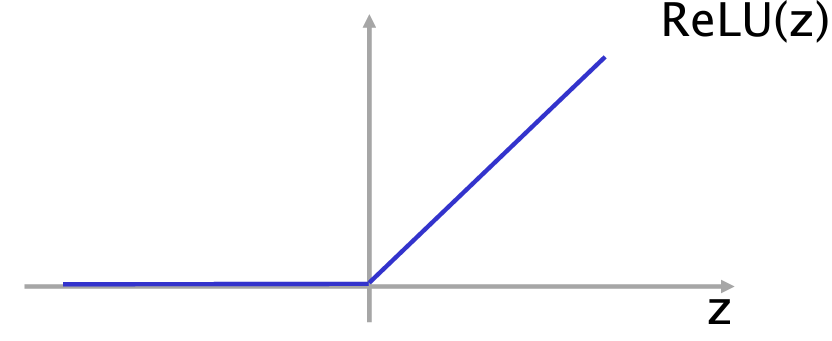
\includegraphics[scale=0.45]{img/ReLU.png}}
    \subfigure[$LeakyReLU(z)=max(\varphi{z}, z)$]{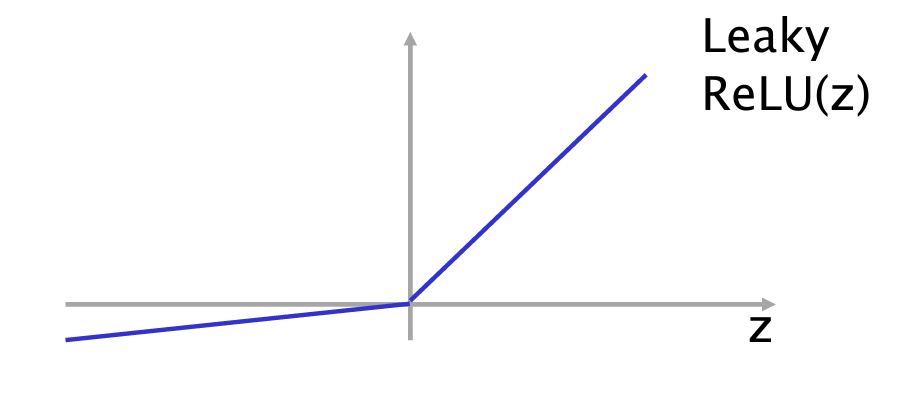
\includegraphics[scale=0.45]{img/LeakyReLU.png}}
    \caption{Some activation functions}
\end{figure}
\noindent
Note that in the $LeakyReLU(z)$ there is a parameter $\varphi$, this is in order to deal with the fact that the derivatives of $ReLU(z)$ for $z<0$ is equal to zero. Such an $\varepsilon$ becomes an hyperparameter.

\section{Initialization of the parameters}
When we have seen the \textit{linear regression} and the \textit{logistic regression}, we have said that the parameters $\theta_i$ would have been initialized for example to zero. This does not work in the case of neural networks. It has been demonstrate that the \textbf{zero-Initialization} of the weights leads to a problem of \textbf{Symmetric weights}, that is after each update, parameters associated to the inputs going to the next hidden layer unit are \textit{identical}. One possible solution, at least for simple NN, is to iniatialize randomly the weights $W^{[l]}$ and biases $b^{[l]}$ with numbers in the interval $[-\epsilon, \epsilon]$. Indeed, more sophisticated approaches are needed in the case of deep neural networks.

\section{Training a neural network (Recipe)}
Once we have presented the main issues related to neural networks and their training, we are ready to give a list of steps aimed to the training: 
\begin{enumerate}
    \itemsep-0.3em
    \item[0.] Pick a network structure, fix the numer of input and output unit with respect to number of inputs and number of classes respectively; the \textit{number of hidden layers} can be decided at this stage and also the number of neurons for each one of such layers. This are all \textbf{hyperparameters}.
    \item Randomly initialize the weights
    \item Implement \textit{forward propagation} in order to get the estimate $\hat{y}^{(i)}$ for any $x^{(i)}$;
    \item Implement code to compute the cost function $J(w,b)$ (this is another choice that we have done according to the task to be performed); 
    \item Implement \textbf{backward propagation} to compute partial derivatives (of the functional wrt the parameters);
    \item Use \textbf{gradient descent} or other optimization methods together with backward propagation to try to minimize $J(w,b)$.
\end{enumerate}

\section{Hyperparameters}
In the field of neural networks is fundamental the distinction between \textbf{parameters} and \textbf{hyperparameters}. The former ones are the ouput of the training phase, they are those that characterize a model from another. The latter ones are related to the choices that the \textit{machine learning engineer} makes in order to improve the performances of the predictive model. Examples of hyperparameters are:
\begin{itemize}
    \itemsep-0.3em
    \item Learning rate $\alpha$ of the gradient descent; 
    \item Number of iterations of the optimization algorithm; 
    \item Number of hidden layers and for each one the number of computational units; 
    \item Activation functions for each layer and related hyperparameters (eg. in the Leaky ReLU there is $\varphi$ to choose)
 \end{itemize}
 The \textbf{optimal (in some sense) configuration} must be found. 

\section{Training, Development, Test sets}
When we want to build a machine learning model, we must have a \textbf{dataset}. Clearly, since the optimal configuration of the network has to be found, only a portion of this data is used for the training phase. In general the dataset is divided into three portions:
\begin{figure}[h]
    \centering
    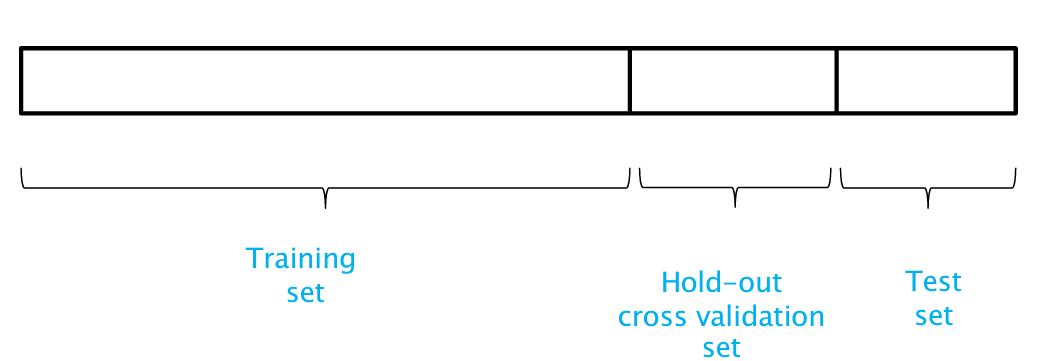
\includegraphics[scale=0.5]{img/dataset.png}
    \caption{Traditional dataset partitioning}
\end{figure}

In the past, when not too much data was available the ratios were 60\%, 20\%, 20\%; however with the increasing of the data availability the trend is using as much data as possible for the training set (98\%) and the remaining part for development and test (1\% for each one).
 \begin{description}
    \item[Training set] Is the biggest part of the dataset which is used for building the model (obtaining parameters). On this set could be necessary preliminary operations of \textit{data preparation} (eg. normalization, data augmentation and so on).
    \item[Cross-Validation/Development set] Is the set used for evaluating different models (not necessarily different architectures, but also different hyperparameters). The data distribution should match with the one in the training set. The validation set which is used, clearly is the same for all the selected models.
    \item[Test set] Once the model has been chosen a test on data that the network has never seen should be done. Such data can be extracted from the dataset, or coming from other sources making optional the presence of this type of set.
\end{description}